\documentclass[twocolumn, a4paper, 10pt]{article}
\usepackage{ctex}

% --- 中文支持 ---
\usepackage[T1]{fontenc}
\usepackage{lmodern}

% --- 页面设置 ---
\usepackage[left=1.5cm, right=1.5cm, top=2cm, bottom=2cm]{geometry}

% --- 数学公式支持 ---
\usepackage{amsmath}
\usepackage{amssymb}
\usepackage{amsfonts}

% --- 图片插入支持 ---
\usepackage{graphicx}

% --- TikZ 绘图 ---
\usepackage{tikz}
\usetikzlibrary{arrows.meta, positioning, calc, shapes.geometric, fit, backgrounds}

% --- 链接与引用 ---
\usepackage[colorlinks, linkcolor=blue, anchorcolor=blue, citecolor=green]{hyperref}

% --- 标题格式调整 ---
\usepackage{titlesec}

% --- 算法伪代码 ---
\usepackage{algorithm}
\usepackage{algpseudocode}
\usepackage{float}
\usepackage{dblfloatfix}
\usepackage{multirow}

\title{\textbf{基于图 Transformer 增强的几何过滤增广轮廓树}\\[6pt]
  \large\textmd{Geometric Filtered Augmented Contour Tree via Graph Transformer Enhancement}}
\author{}
\date{}

\begin{document}
\raggedbottom
\sloppy
\setlength{\emergencystretch}{2em}
\hbadness=10000
\setlength{\parindent}{2em}
\setlength{\parskip}{0pt}

\maketitle

\begin{abstract}
增广轮廓树通过在临界节点之间插入大量普通节点来记录等值面的连续演化，但相邻普通节点对应的等值面往往高度相似，造成冗余。现有方法要么依赖手工设计的拓扑权重做简化而忽略分支内部的几何演化，要么度量几何相似性却脱离轮廓树分支结构。本文提出一种拓扑保持的几何过滤增广轮廓树节点简化框架：在严格保留所有连通性与亏格变化临界点的前提下，以"活性子图"——等值面在底层网格上的离散截交结构——作为统一的几何描述子，给出 Jaccard 边集距离与基于 SAT+GPS 图 Transformer 编码的向量化距离两种可替换度量，并通过多分支加权贪心算法沿拓扑分支筛选几何上有代表性的节点。在 20 个合成标量场数据集上的实验表明，SAT+GPS 增强度量在对称 Chamfer 距离、Hausdorff 距离和面积属性误差等中立指标上分别改善纯 Jaccard 基线 4.84\%、4.28\% 和 4.19\%，且在未参与训练的测试子集上改善幅度更大。
\end{abstract}

\section{引言}

科学计算、医学影像和流体模拟产生的三维标量场中，等值面是刻画场结构的基本工具。\cite{lorensen_cline_1987} 选择有代表性的等值面——覆盖不同的空间区域、拓扑事件与几何形态——对于数据分析与可视化至关重要。轮廓树（contour tree）\cite{van_kreveld_1997,carr_contour_2003} 通过记录等值面连通分量随阈值变化的出生、合并、分裂与消亡过程，为等值面的全局层次结构提供了紧凑的拓扑描述。增广轮廓树\cite{gueunet_act_2019} 进一步在临界节点之间插入大量普通节点以记录中间等值面状态，但这也带来了显著的冗余：相邻普通节点对应的等值面往往在几何上高度相似。

如何在保留关键拓扑信息的前提下去除这种冗余，是一个尚未被充分解决的问题。拓扑方法（如基于持久性的分支剪枝\cite{edelsbrunner_persistence_2002,carr_geometric_2004}）能保住连通性与亏格变化的临界点，却难以刻画同一拓扑分支内部等值面几何形状的演化；几何方法（如等值面相似性图 ISM\cite{bruckner_ism_2010}）能度量形状差异，却脱离轮廓树的分支结构，将多个连通分支的变化混合到同一描述符中。两类方法尚未在同一框架内统一。

本文提出一种基于几何过滤的增广轮廓树节点简化框架，在三个层面同时保障等值面序列的代表性：（1）\textbf{拓扑保持}：所有结构节点（极值点、鞍点、分支节点）无条件保留，Morse 理论保证的亏格不变区间约束使分支内部仅做纯几何筛选；（2）\textbf{几何感知}：以"活性子图"——等值面在底层网格上的离散截交结构——作为统一描述子，给出 Jaccard 边集差异与基于图 Transformer 编码的向量化差异两种可替换度量；（3）\textbf{多分支感知}：同一标量层级穿过的多条分支按拓扑显著性与几何规模加权聚合。其中图 Transformer 编码器采用 GraphGPS\cite{rampasek_gps_2022} 框架为骨架，引入 SAT\cite{chen_sat_2022} 风格的结构感知注意力（query 与 key 取自局部消息传递输出而非原始节点特征），并以活性边上的等值面插值参数作为连续边特征，使编码器能够捕捉 Jaccard 二值边集所不具备的几何信息。

值得强调的是，本框架中学习组件被严格限制在几何通道内：拓扑保持（结构节点保留、亏格区间划分）和最终的贪心判定均为确定性算法，不经过神经网络；编码器仅在"分支内部拓扑已保证不变"的前提下度量几何差异。因此，无论编码器的训练效果如何，拓扑正确性均不受影响。

在 20 个规则网格合成标量场数据集上的实验表明：（1）结构节点保留率恒为 100\%，简化强度可由单一参数 $\varepsilon$ 连续控制；（2）SAT+GPS 增强度量在对称 Chamfer 距离、Hausdorff 距离等中立几何指标上分别改善纯 Jaccard 基线 4.84\% 和 4.28\%，且在未参与编码器训练的测试子集上改善幅度更大（Chamfer $-10.2\%$，Hausdorff $-7.6\%$）；（3）多分支加权在分支重叠度适中的数据上提升最小分支保留率，改善覆盖均匀性。

\section{相关研究与研究动机}

本节按”背景—研究动机—相关研究”的顺序展开：\ref{sec:background} 节给出等值面、轮廓树及其亏格、欧拉示性数与连通性的学术化背景；\ref{sec:motivation} 节从”选择代表性等值面”出发引出本文方法；\ref{sec:related} 节梳理已有的拓扑与几何两类工作。

\subsection{背景}
\label{sec:background}

\paragraph{等值面}科学计算、医学影像和流体模拟中的数据常表示为定义在空间域上的标量场 $f:\Omega\rightarrow\mathbb{R}$。给定标量阈值 $\alpha$，其等值面（isosurface）定义为原像 $f^{-1}(\alpha)=\{x\in\Omega\mid f(x)=\alpha\}$，在三维标量场中一般是一张或多张独立的封闭曲面。Marching Cubes 等方法可在规则网格上把 $f^{-1}(\alpha)$ 显式重建为三角网格（triangle mesh），是流场可视化分析中刻画结构的基本工具。\cite{lorensen_cline_1987} 然而逐阈值抽取只能给出孤立层级的几何，难以揭示等值面随阈值连续变化时的全局层次结构。

\paragraph{轮廓树}拓扑数据分析为此提供了更紧凑的表示。轮廓树（contour tree）通过刻画等值面连通分量随阈值变化的演化，把连续阈值空间压缩为一棵树：它记录等值面 $f^{-1}(\alpha)$ 的连通分量随阈值 $\alpha$ 变化而出生、合并、分裂与消亡的过程。\cite{van_kreveld_1997,carr_contour_2003} 形式上，它可由记录子水平集 $F_\alpha=\{x\in\Omega\mid f(x)\leq\alpha\}$ 连通分量演化的并树（join tree）与记录超水平集演化的分裂树（split tree）合并得到。极值点、鞍点和分支节点对应关键拓扑事件，树边则表示相邻事件之间的演化区间。Topology ToolKit（TTK）等工具已将这些结构封装为可与 ParaView、VTK 衔接的工程模块，为轮廓树的计算与增广提供了标准实现。\cite{tierny_ttk_2018}

\paragraph{等值面的亏格与欧拉示性数}等值面的亏格（genus）$g$ 在拓扑学上的直观含义是一张闭合、可定向曲面上所含“把手”（handles）或“孔洞”（holes）的数量，是刻画其复杂程度的核心拓扑不变量：$g=0$ 对应球面，$g=1$ 对应环面（如甜甜圈或带一个把手的杯子），$g=2$ 对应双环面，$g=n$ 则对应带 $n$ 个相互独立把手的曲面。亏格亦可由 Betti 数刻画——对一张连通闭合可定向曲面，$0$ 维 Betti 数 $\beta_0=1$ 计连通分量、$1$ 维 Betti 数满足 $\beta_1=2g$、$2$ 维 Betti 数 $\beta_2=1$——从而把“把手数”与曲面上独立环路的数量联系起来。\cite{edelsbrunner_harer_2010} 对由 Marching Cubes 抽取的三角网格，亏格通过网格的点、边、面数量联合定义。对一个连通且闭合的等值面网格，其欧拉示性数（Euler characteristic）为
\begin{equation}
\chi = V - E + F,
\label{eq:euler}
\end{equation}
其中 $V,E,F$ 分别为顶点、边、三角面片总数。由拓扑学定理，欧拉示性数与亏格满足线性关系
\begin{equation}
\chi = 2 - 2g,\qquad g = \frac{2-\chi}{2}.
\label{eq:genus}
\end{equation}
若同一阈值下抽取出 $c$ 个彼此不相连的独立封闭曲面（各自亏格之和为 $g$），则关系修正为 $\chi=2c-2g$，即 $g=(2c-\chi)/2$。因此，只要能沿阈值追踪 $\chi$ 的变化，就能反推等值面的亏格演化。

\paragraph{轮廓树与等值面亏格的关系}轮廓树本身无法完全表达等值面的亏格——它记录连通分量的演化，却不直接给出每张曲面上“把手”的数量，两个亏格截然不同的等值面在轮廓树上可能共享完全相同的边。\cite{carr_flexible_2010} 但亏格的变化严格遵循 Morse 理论：\cite{milnor_morse_1963,edelsbrunner_harer_2010} 只有当阈值 $h$ 穿过轮廓树的节点（临界点）时等值面的拓扑才会跳变，且每个临界点对欧拉示性数的贡献由其 Morse 指数 $i$ 决定——指数 $i$ 的临界点使 $\chi$ 改变 $(-1)^i$。在三维标量场中，$i=0$（极小值）与 $i=3$（极大值）对应等值面连通分量的出生与消亡，$i=1$ 与 $i=2$ 的鞍点则对应亏格的改变：当等值面在两处相交、在中间形成一条通道（环）时亏格加一，对应一阶鞍点（$1$-saddle）；当通道闭合时亏格减一，对应二阶鞍点（$2$-saddle）。据此，已有工作可在轮廓树的极小值边上初始化 $\chi$，沿阈值扫掠在每个节点按其类型累加贡献，从而在保留树结构的同时把亏格信息补全到树的每条边上；实际数据中常出现的多重（非 Morse）鞍点需先经虚拟扰动拆解为标准一阶、二阶鞍点组合，才能保证贡献累加正确。\cite{van_kreveld_1997,carr_contour_2003,ni_fair_2004} 本文不显式计算亏格，仅将上述关系作为说明等值面代表性、并论证“树边内部拓扑不变”的理论背景。

\begin{table}[h]
\centering
\small
\caption{三维标量场中各类临界点（Morse 指数 $i$）对等值面欧拉示性数 $\chi$ 的贡献 $\Delta\chi=(-1)^i$。连通分量数 $c$ 与亏格 $g$ 的净变化再由 $\chi=2c-2g$ 统一反推——同一 $\Delta\chi$ 可能来自连通性事件或亏格事件，需结合分量数区分。}
\label{tab:critical}
\begin{tabular}{ccl}
\hline
类型 & $\Delta\chi$ & 主要拓扑含义 \\
\hline
极小值（$i=0$） & $+1$ & 连通分量出生（$c$ 增） \\
一阶鞍点（$i=1$） & $-1$ & 连通分量合并，或生成通道使 $g$ 增 \\
二阶鞍点（$i=2$） & $+1$ & 连通分量分裂，或通道闭合使 $g$ 减 \\
极大值（$i=3$） & $-1$ & 连通分量消亡（$c$ 减） \\
\hline
\end{tabular}
\end{table}

\paragraph{轮廓树与等值面连通性的关系}若说亏格描述单张曲面的复杂程度，连通性则描述等值面在阈值扫掠中的整体演变，而轮廓树正是这一演变的“家谱”：它追踪并记录等值面在不同阈值下的连通分量如何诞生、合并、分裂与消失。轮廓树的节点恰是连通性发生改变的临界时刻——阈值经过极小值点时诞生一个新的连通分量，经过极大值点时一个连通分量收缩为点而消失；鞍点则是连通分量重组之处：一个分量被“扯断”为两个（分裂），或两个原本独立的分量“黏连”为一个（合并）。这一背景表明，等值面的连通性与亏格变化都被编码在轮廓树的结构节点（极值点与鞍点）上，而树边内部则是拓扑不变的演化区间。

\begin{figure*}[t]
\centering
\begin{tikzpicture}[
    node distance=0.6cm and 0.5cm,
    box/.style={rectangle, draw=black!70, fill=blue!6, thick, rounded corners=3pt,
                minimum height=0.9cm, minimum width=2.4cm, align=center,
                font=\small\sffamily},
    arrow/.style={-{Stealth[length=2mm, width=1.8mm]}, thick, draw=black!70},
    label/.style={font=\tiny\sffamily, text=black!60, align=center},
]
% 主流程节点
\node[box] (input) {输入\\[-1pt]{\tiny 标量场 $f$ + 增广轮廓树 $T$}};
\node[box, right=of input] (weight) {多分支权重\\[-1pt]{\tiny 持久性权重 + 规模权重}};
\node[box, right=of weight] (genus) {亏格不变区间\\[-1pt]{\tiny 分支内拓扑不变保证}};
\node[box, right=of genus] (geo) {几何差异度量\\[-1pt]{\tiny Jaccard + SAT+GPS / $\lambda$ 残差}};
\node[box, right=of geo] (greedy) {贪心简化\\[-1pt]{\tiny 链上扫描, 阈值判定}};
\node[box, right=of greedy] (output) {输出\\[-1pt]{\tiny 简化树 $T'$}};

% 箭头
\draw[arrow] (input) -- (weight);
\draw[arrow] (weight) -- (genus);
\draw[arrow] (genus) -- (geo);
\draw[arrow] (geo) -- (greedy);
\draw[arrow] (greedy) -- (output);

% 节标注
\node[label, above=0.15cm of weight] {\S\ref{sec:branch-weight}};
\node[label, above=0.15cm of genus] {\S\ref{sec:genus-interval}};
\node[label, above=0.15cm of geo] {\S\ref{sec:geo-repr}};
\node[label, above=0.15cm of greedy] {\S\ref{sec:greedy}};
\end{tikzpicture}
\caption{方法流程图。输入标量场与增广轮廓树，经多分支权重计算、亏格不变区间约束、分支几何差异度量（Jaccard + SAT+GPS 编码 + $\lambda$ 对齐残差），最终通过贪心简化算法输出几何过滤增广轮廓树。}
\label{fig:pipeline}
\end{figure*}

\subsection{研究动机}
\label{sec:motivation}

等值面是流场可视化分析中的重要工具，选择有代表性的等值面对于刻画流场特征具有重要意义。一张等值面是否具有代表性，可从三个方面衡量。其一是等值面的位置与分布：代表性的等值面应覆盖标量场中不同的空间区域与阈值层级，避免集中于单一区间而遗漏其他特征区域。其二是等值面的连通性以及亏格变化：如 \ref{sec:background} 节所述，连通分量的出生、合并、分裂、消亡以及亏格的增减都被编码在轮廓树的极值点与鞍点上，代表性的等值面序列应完整覆盖这些拓扑事件。其三是等值面的几何特征：即便拓扑不变，等值面的形状、规模与截穿的局部结构仍可能明显演化，代表性应捕捉这类几何差异。前两个方面主要与拓扑分析和简化相关，其代表工作是轮廓树、合并树以及 Carr 等的柔性等值面框架；\cite{carr_contour_2003,carr_flexible_2010,gueunet_act_2019} 第三个方面主要与 ISM 等几何方法相关。\cite{bruckner_ism_2010} 然而如 \ref{sec:related} 节所述，拓扑方法能保住连通性与亏格变化点却难以刻画分支内几何演化，几何方法能度量形状差异却常脱离轮廓树分支、混合多分支变化，现有研究因而并不能真正选出有代表性的等值面，也没有方法同时针对上述三个方面。

本文正是为弥合这一空缺而提出。我们把”选择代表性等值面”具体化为增广轮廓树上的节点筛选问题：为在连续阈值上保留代表性的等值状态，增广轮廓树在临界节点之间插入大量普通节点，\cite{gueunet_act_2019,lukasczyk_extreem_2023,li_distributed_2024} 但相邻普通节点对应的等值结构往往高度相似，造成冗余——保留全部普通节点会产生近似重复的等值面并增加存储与交互成本，而不加区分地删除又会丢失真实的几何演化。本文在严格保留关键拓扑结构（根、叶、鞍点与分支节点，即连通性与亏格变化的临界点，见 \ref{sec:background} 节）的前提下，沿拓扑分支筛选出几何上有代表性的普通节点，从而在位置分布、连通性与亏格、几何特征三个层面同时逼近原始等值面序列。

这一目标落实为三项设计。其一，简化范围受拓扑约束：结构节点全部保留，候选普通节点沿所属拓扑分支顺序筛选，简化后通过合并原始弧重建合法树，从而保住连通性与亏格变化所依附的结构节点。其二，基础差异度量按分支实例化：本文统一以原始网格上的局部活性子图刻画分支局部结构，并给出两种可替换的比较方式——活性边集合的 Jaccard 距离与活性子图的 SAT+GPS 向量化距离，分别从显式边集与图 Transformer 结构编码两个角度度量几何差异。其三，多分支场景下按重要性加权：一个标量层级可能同时穿过主分支与旁支，本文保留这些分支身份，并按标量跨度型拓扑显著性与几何规模把多个分支的差异汇总为整体差异。据此，本文提出一个拓扑保持的多分支感知增广轮廓树节点简化框架。

\subsection{相关研究}
\label{sec:related}

围绕等值面表示与轮廓树简化的已有工作可从三个方面梳理：拓扑驱动的合并树与轮廓树简化方法、几何驱动的等值面相似性度量方法，以及面向网格数据的图表示学习方法。

Van Kreveld 等最早将轮廓树引入等值面遍历，以其变体构造可证明规模最小的种子集从连通分量中精确提取等值面。\cite{van_kreveld_1997} Carr 等提出通过合并 Join 树与 Split 树的通用维度轮廓树算法，成为轮廓树计算的标准参考实现。\cite{carr_contour_2003} Edelsbrunner 等引入持久同调，以特征在过滤中的存活时间区分信号与噪声，奠定多尺度拓扑简化的理论基础。\cite{edelsbrunner_persistence_2002} Carr 等为轮廓树分支引入面积、体积以及兼顾空间规模与函数值偏离的超体积等局部几何度量，作为分支剪枝的代价函数；\cite{carr_geometric_2004} 在此基础上又提出柔性等值面框架，以轮廓树分支索引独立 contour，并结合叶子剪枝与顶点归约实现交互式简化与显示，是本文最直接的相关工作。\cite{carr_flexible_2010} 面向并行计算，Gueunet 等提出基于 Fibonacci 堆的任务并行增广轮廓树算法，是本文简化工作的直接操作对象；\cite{gueunet_act_2019} Lukasczyk 等以极值图为骨架提出 ExTreeM，进一步降低增广合并树并行计算的串行开销。\cite{lukasczyk_extreem_2023} Tierny 等开发 Topology ToolKit（TTK），为合并树、轮廓树、Morse-Smale 复形等拓扑结构提供开源标准实现。\cite{tierny_ttk_2018} 在分布式与大规模场景下，Li 等先将增广、超扫掠与分支分解扩展到分布式环境，使分布式轮廓树可作为科学探索的查询结构，\cite{li_distributed_2024} 后进一步引入预简化策略，在数百亿网格元素上完成层次化轮廓树的构造。\cite{li_presimplification_2025} 在合并树相似性度量方向，Sridharamurthy 与 Natarajan 提出局部树编辑距离，把整树比较推进到子结构级；\cite{sridharamurthy_local_2021} Wetzels 等把 Wasserstein 测地线/重心与路径映射编辑距离结合，得到分支分解无关的鲁棒度量；\cite{wetzels_path_2023} Pont 与 Garth 进一步引入区域感知 Wasserstein 距离，把极值对齐区域的取值分布显式纳入度量。\cite{pont_region_2025} 这些方法与本文均以"分支/子结构 + 几何信息"为共同切面，但仍以手工设计的持久性/几何权重作为过滤依据，缺少对局部几何结构本身的表达能力。

Bajaj 等提出等值面谱（contour spectrum），将等值面面积、体积、梯度积分等属性表达为等值的分段 B 样条函数，首次将几何量化方法引入等值面阈值选择。\cite{bajaj_spectrum_1997} Chiang 与 Lu 提出保持所有可能等值面拓扑的渐进四面体网格简化算法，是拓扑感知网格简化的关键先驱。\cite{chiang_lu_2003} Bruckner 与 Möller 提出等值面相似性图（ISM），以归一化互信息比较不同阈值下的距离场结构，从相似度矩阵中选出代表性等值面，是等值面几何相似性度量的里程碑；\cite{bruckner_ism_2010} 但 ISM 将多个连通分支的变化混合到同一距离场描述符中，难以区分分支级别的几何差异。Wang 提出基于区间体与等值面面积的 VOA 度量以及基于点距的分割度量，用于自动检测代表性等值与语义化等值面分割。\cite{wang_isomeasure_2020} 在此基础上，Li 等将 ISM 扩展到多视图场景，通过跨视图一致的相似性聚类同时驱动传递函数设计与代表性等值面选择；\cite{li_multiview_ism_2025} Zhou 等面向气象集合数据，以 contour probability similarity 做非均匀下采样得到 key-isovalue，并结合信息损失曲线自动决定采样密度。\cite{zhou_keyisovalue_2025} 深度表征方面，Dai 等提出 IsoExplorer，用 Octree 卷积变分自编码器学习每张连通等值面的潜表示，把等值面相似性从"距离场互信息"迁移到"神经嵌入距离"；\cite{dai_isoexplorer_2021} He 等则提出 ScalarGCN，把标量值作为图节点用 GCN 学习关联表征，是把 GCN 系统性引入体数据分析的先驱之一。\cite{he_scalargcn_2021} Li 与 Shen 借助不确定度传播，把隐式神经表示上的等值面提取显著加速，代表神经场表征下的等值面几何提取方向。\cite{li_shen_inr_2024} 上述工作展示了 ISM 家族从"手工描述子"迈向"多视图/集合/神经表征"的演化，但共同短板是脱离轮廓树的分支结构，几何差异被混合在多分支之间。

消息传递图神经网络（MPNN）通过邻域聚合迭代更新节点表示，\cite{gilmer_mpnn_2017} 以 GCN\cite{kipf_gcn_2017} 和 GIN\cite{xu_gin_2019} 为代表，为图表示学习奠定了基础；但其感受野受限于层数，理论判别能力不超过 Weisfeiler-Leman 测试。\cite{xu_gin_2019} 为突破消息传递的局限，图 Transformer（GT）引入全局注意力以直接建模任意节点对的交互。Ying 等提出 Graphormer，以中心度、空间距离与边属性作为注意力偏置，在分子性质预测基准上取得了突破性成绩，是将 Transformer 成功引入图学习的标志性工作。\cite{ying_graphormer_2021} Kreuzer 等提出 SAN（Spectral Attention Network），通过专用的可学习位置编码模块处理 Laplacian 全谱信息，并在注意力中显式区分真实边与虚拟边。\cite{kreuzer_san_2021} Dwivedi 等提出 LSPE，将结构与位置编码解耦为两路并在消息传递中联合更新，而非仅作为固定的输入拼接。\cite{dwivedi_rwse_2022} Lim 等提出 SignNet/BasisNet，构建对 Laplacian 特征向量符号翻转和高维基旋转具有严格不变性的网络，使谱位置编码在理论上良定义。\cite{lim_signnet_2023} 在架构层面，Chen 等提出结构感知 Transformer（SAT），将注意力核从比较节点特征改为比较以节点为中心提取的子图表示，使注意力本身具备结构感知能力，并给出可控性与判别力两条理论保证。\cite{chen_sat_2022} Rampasek 等提出 GraphGPS 通用框架，将 GT 系统拆解为位置/结构编码、局部消息传递与全局注意力三个可替换模块；\cite{rampasek_gps_2022} Kim 等提出 TokenGT，将节点与边均视为独立 token 送入标准 Transformer，证明其表达力不低于 2 阶不变图网络。\cite{kim_tokengt_2022} 面向可扩展性，Shirzad 等提出 Exphormer，结合扩展图与虚拟节点构建稀疏注意力，在线性复杂度下保持谱近似与通用性保证。\cite{shirzad_exphormer_2023} Bar-Shalom 等提出 Subgraphormer，通过图积视角把子图 GNN 与图 Transformer 统一，为"子图提取 + Transformer 编码"范式提供理论表达力支撑。\cite{barshalom_subgraphormer_2024} 面向网格与物理仿真，MeshCNN\cite{hanocka_meshcnn_2019} 和 DiffusionNet\cite{sharp_diffusionnet_2022} 分别在三角网格的边和 Laplace-Beltrami 算子上定义学习操作；Wu 等提出 Transolver，以物理感知的 token 切片替代逐顶点 token，实现面向一般几何的线性复杂度 PDE 求解。\cite{wu_transolver_2024} 在图度量学习方向，Jain 等提出 GRAPHEDX，用神经集散度学习通用代价下的图编辑距离。\cite{jain_graphedx_2024} 与本文最直接相关的工作是 Qin 等提出的合并树神经网络（MTNN），首次系统地用 GNN 学习整棵合并树的相似度嵌入，将拓扑比较速度提升两个数量级；\cite{qin_mtnn_2024} 但 MTNN 学习的是"整棵合并树"的相似度嵌入用于比较任务，而本文用图 Transformer 学习"分支级活性子图"的向量化用于增广轮廓树的几何过滤，输入图结构、监督信号与下游任务均不同，两者是"图表示学习 + 拓扑抽象"方向的两个互补切面。

综上，拓扑方法能保住连通性与亏格变化点却难以刻画分支内几何演化，几何方法能度量形状差异却脱离轮廓树分支结构，图表示学习提供了局部结构编码的工具但尚未应用于等值面代表性筛选。三者尚未在同一框架内统一，这一空缺正是本文工作的出发点。
\section{方法}

本节给出基于几何过滤的增广轮廓树节点简化方法。输入为规则网格 $\Omega$ 上的标量场 $f:\Omega\rightarrow\mathbb{R}$ 及其增广轮廓树 $T=(V,E,f)$，输出为几何过滤增广轮廓树 $T'$——在严格保留连通性与亏格变化临界点的前提下，沿拓扑分支筛选出几何上有代表性的普通节点后重建而得的简化树。图~\ref{fig:pipeline} 给出方法的整体流程；图~\ref{fig:framework} 给出核心概念的直观示意——增广轮廓树的临界点将标量轴划分为若干亏格不变区间，每条拓扑分支对应一个区间，分支内部等值面拓扑不变、仅有几何演化。全文按以下逻辑展开：\ref{sec:branch-weight} 节定义多分支权重；\ref{sec:genus-interval} 节说明亏格不变区间；\ref{sec:geo-repr} 节给出两种几何差异度量；\ref{sec:greedy} 节统一为贪心简化算法。

\begin{figure*}[t]
\centering
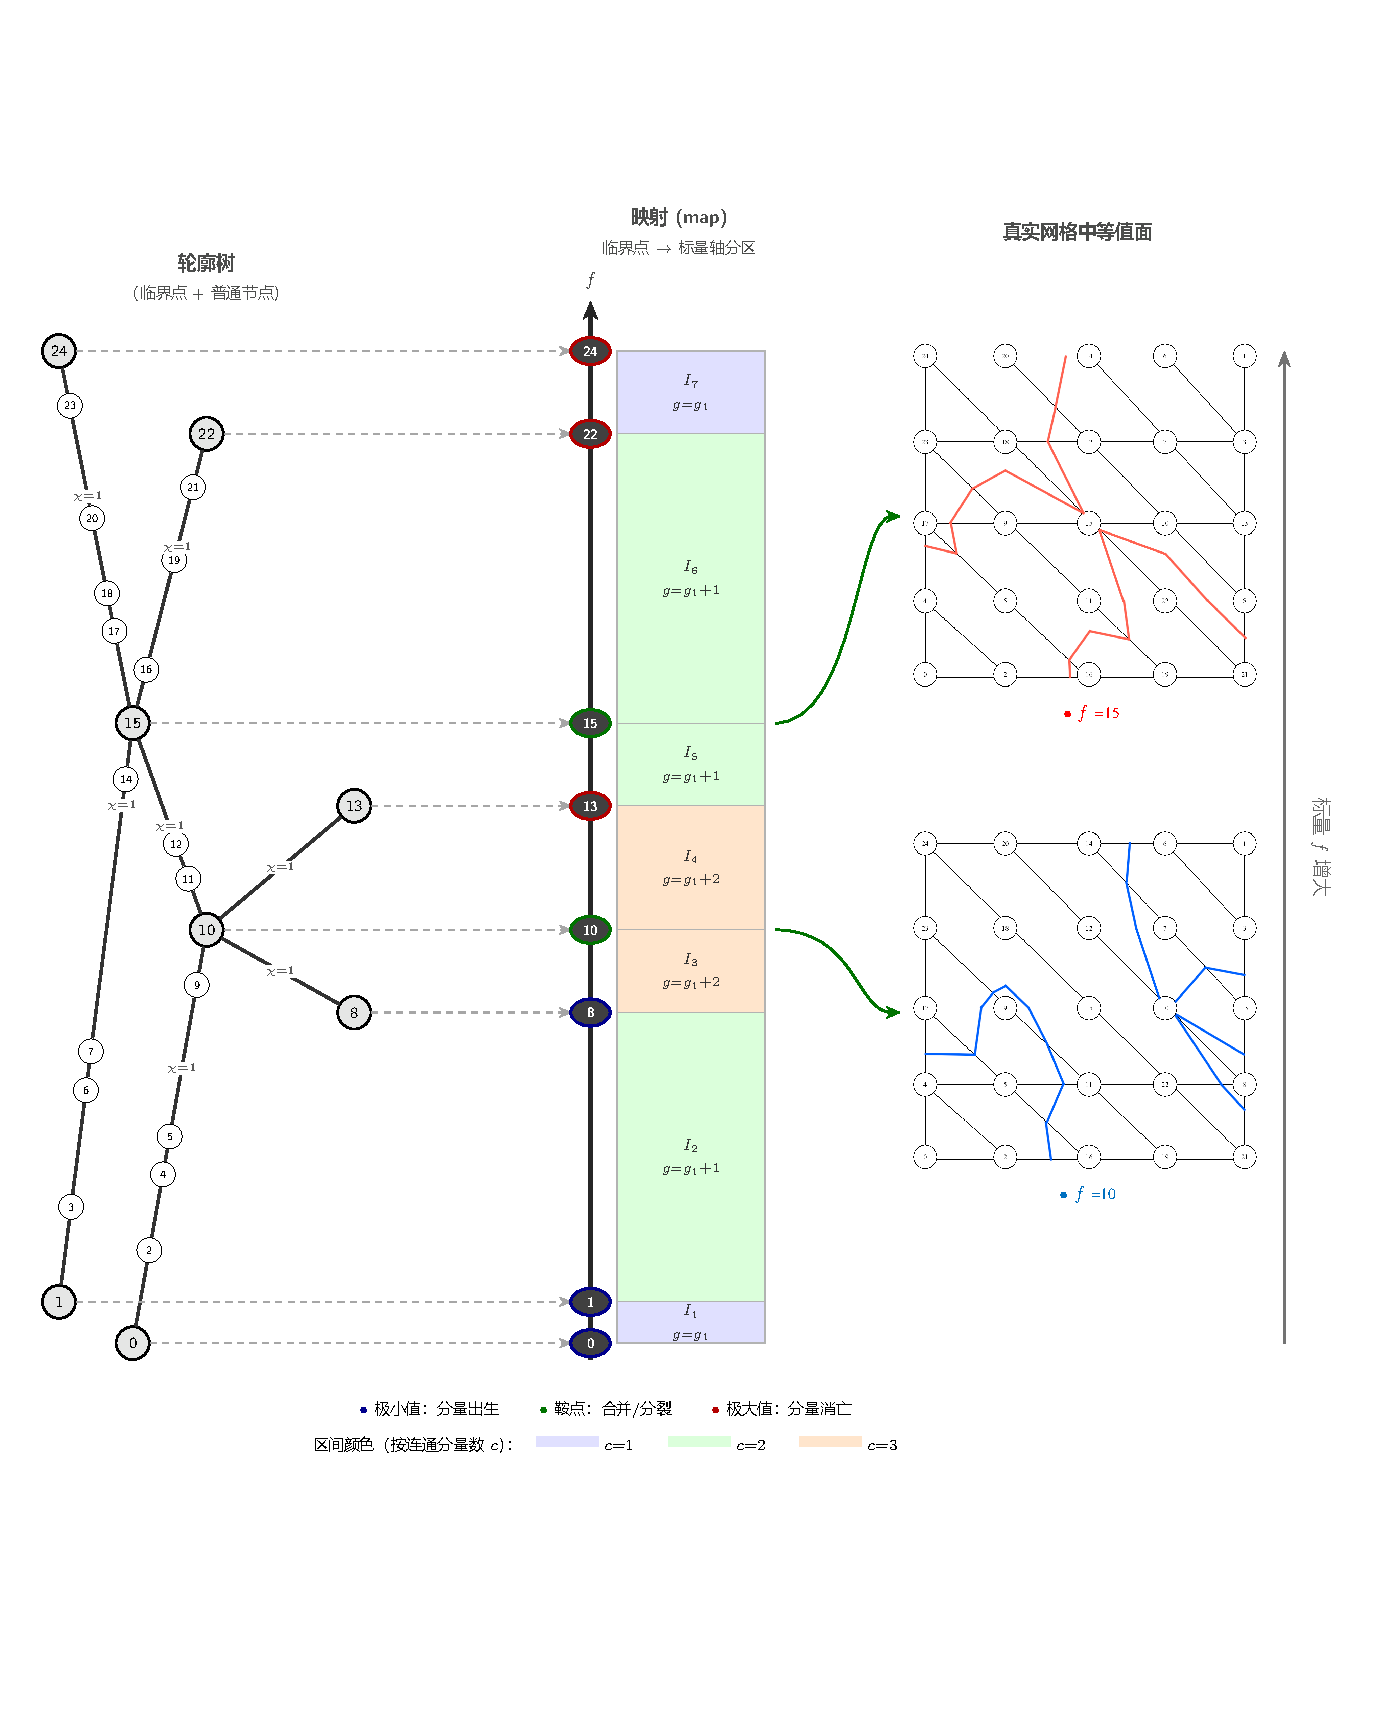
\includegraphics[height=0.42\textheight]{fig-framework.pdf}
\caption{增广轮廓树到临界值分区映射。左：轮廓树（灰色圆为结构节点即临界点，白色圆为普通节点）；中：临界点沿等高度投影到标量轴 $f$，将其划分为若干区间 $I_1$--$I_7$；右：在鞍点处提取的真实网格等值面，展示分量合并瞬间。图中颜色按连通分量数 $c$ 区分（蓝色 $c{=}1$，绿色 $c{=}2$，橙色 $c{=}3$）；临界点类型以边框颜色标记（蓝=极小值/分量出生，绿=鞍点/合并或分裂，红=极大值/分量消亡）。各区间内亏格 $g$ 保持不变：设 $I_1$ 亏格为 $g_1$，则 $g = g_1 + (c-1)$；$\chi$ 为边/区间等值面的 Euler 示性数。}
\label{fig:framework}
\end{figure*}

% ========================================
% 3.1 多分支权重
% ========================================
\subsection{多分支权重}
\label{sec:branch-weight}

增广轮廓树的节点按拓扑角色分为\textbf{结构节点}与\textbf{普通节点}两类（如图~\ref{fig:framework} 左部所示）。结构节点集合 $V_s$ 包含根、叶（极值点）和分支节点（鞍点），记录连通性与亏格的跳变；普通节点集合 $V_o = V \setminus V_s$ 为度数等于~$2$ 的增广节点，记录中间等值面状态。相邻结构节点之间由普通节点串连而成的路径称为一条\textbf{拓扑分支}（topological branch）$b_\ell = (v_0, v_1, \ldots, v_k)$，其中端点 $v_0, v_k \in V_s$，中间节点按标量值排列。每条分支的\textbf{标量跨度}（scalar span）定义为
\[
\pi_\ell = f_{\max}(b_\ell) - f_{\min}(b_\ell),
\]
它刻画该分支承载的标量演化范围，在拓扑数据分析中对应\textbf{持久性}（persistence）在分支层面的近似——持久性衡量一个拓扑特征在过滤中的存活时间，$\pi_\ell$ 越大表示分支承载的演化区间越长，在简化中应越被优先保护。

在轮廓树中，同一标量层级 $t_i = f(v_i)$ 可能同时穿过多条拓扑分支。记活跃分支集合为
\begin{equation}
\mathcal{B}(t_i) = \{\,b_\ell \mid f_{\min}(b_\ell) \leq t_i \leq f_{\max}(b_\ell)\,\}.
\label{eq:active-branch}
\end{equation}
节点筛选需同时考虑所有活跃分支的变化，为此对每条活跃分支 $b_\ell$ 定义两类权重。\textbf{拓扑权重} $w^{\mathrm{topo}}_\ell$ 按标量跨度归一化，使跨度越大的分支获得更高权重；\textbf{几何规模权重} $w^{\mathrm{geo}}_\ell$ 按该分支在参考节点与候选节点之间的活性边规模变化归一化——记参考节点 $v_r$ 与候选节点 $v_i$ 在分支 $b_\ell$ 上的活性边数分别为 $s_{r,\ell}$ 和 $s_{i,\ell}$（定义见 \ref{sec:geo-repr} 节），先计算相对规模变化 $g_\ell = |s_{r,\ell} - s_{i,\ell}|/\max(s_{r,\ell},\,\epsilon_0)$，再归一化，使规模变化越大的分支获得更高权重：
\begin{equation}
w^{\mathrm{topo}}_\ell = \frac{\pi_\ell}{\sum_{k:\,b_k \in \mathcal{B}(t_i)} \pi_k},\qquad
w^{\mathrm{geo}}_\ell = \frac{g_\ell}{\sum_{k:\,b_k \in \mathcal{B}(t_i)} g_k}.
\label{eq:weights}
\end{equation}
二者通过混合系数 $\alpha \in [0,1]$ 线性组合为最终权重
\begin{equation}
w_\ell = \frac{\alpha\,w^{\mathrm{topo}}_\ell + (1-\alpha)\,w^{\mathrm{geo}}_\ell}
{\sum_{k}\bigl[\alpha\,w^{\mathrm{topo}}_k + (1-\alpha)\,w^{\mathrm{geo}}_k\bigr]}.
\label{eq:wmix}
\end{equation}
$\alpha = 1$ 退化为纯拓扑权重，倾向保护持久性高（标量跨度大）的主分支，但可能低估正经历显著截交变化的旁支；$\alpha = 0$ 退化为纯几何规模变化权重，响应参考与候选之间的局部结构变化但可能稀释拓扑上重要的小分支。各活跃分支的局部差异 $d_\ell$（定义见 \ref{sec:geo-repr} 节）经权重汇总为整体差异
\begin{equation}
D(v_r, v_i) = \sum_{\ell:\,b_\ell \in \mathcal{B}(t_i)} w_\ell\, d_\ell(v_r, v_i),\qquad \sum_\ell w_\ell = 1,
\label{eq:aggregate}
\end{equation}
其中 $v_r$ 为当前分支链上最近一次保留的参考节点，$v_i$ 为待判定的候选节点，$d_\ell(v_r, v_i)$ 为分支 $b_\ell$ 上从 $v_r$ 到 $v_i$ 的几何差异。$D$ 是贪心简化（\ref{sec:greedy} 节）中决定是否保留 $v_i$ 的核心判据：当 $D$ 超过阈值时保留 $v_i$，否则跳过。

% ========================================
% 3.2 亏格不变区间与分支映射
% ========================================
\subsection{亏格不变区间与分支映射}
\label{sec:genus-interval}

Morse 理论保证：只有当阈值穿过轮廓树的临界点（结构节点）时等值面的拓扑才发生跳变，每个临界点对欧拉示性数的贡献为 $\Delta\chi=(-1)^i$（$i$ 为 Morse 指数）。因此，在两个相邻结构节点之间的标量区间内，等值面的连通分量数和亏格均保持不变。如图~\ref{fig:framework} 中部所示，临界点沿等高度投影到标量轴后将其划分为若干区间 $I_1$--$I_7$，每个区间对应一条拓扑分支 $b_\ell=(v_0,\ldots,v_k)$，其端点 $v_0,v_k\in V_s$ 之间的开区间 $(f(v_0),f(v_k))$ 不含其他临界点，即为一个\textbf{亏格不变区间}（genus-invariant interval）。在此区间内，等值面的拓扑类型不随阈值变化，只有几何形状可能演化——这正是在分支内部做纯几何筛选的理论基础。

这一映射具有三方面关键保证：（1）分支内部拓扑不变——任意两个普通节点的等值面具有相同的连通分量数和亏格，二者差异纯粹是几何差异；（2）亏格变化仅发生在端点——如图~\ref{fig:framework} 右部所示，鞍点处等值面发生分量合并或分裂，一阶鞍点使亏格增加、二阶鞍点使其减少，本文通过保留所有结构节点来保证亏格变化点不被删除；（3）分支间互不干涉——同一层级穿过的多条分支各自对应独立的亏格不变区间，几何比较被严格限制在各分支内部（\ref{sec:geo-repr} 节）。

综合以上，结构节点全部保留确保不丢失任何亏格变化事件；分支内部仅做几何筛选，不会引入或遗漏拓扑事件；多分支加权保持各分支的独立性，不跨越亏格不变区间混合比较。这一设计使学习组件被严格限制在几何通道内——编码器仅在"拓扑已保证不变"的分支内部度量几何差异，不参与拓扑判定；因此，无论编码器的训练效果如何，拓扑正确性均不受影响。

% ========================================
% 3.3 分支上的几何表示学习
% ========================================
\subsection{分支上的几何表示学习}
\label{sec:geo-repr}

由 \ref{sec:genus-interval} 节可知，拓扑分支内部等值面的差异纯粹是几何差异。本节定义统一的局部结构描述子——活性子图，并给出两种可替换的差异度量。

\subsubsection{局部活性子图}
\label{sec:subgraph}

Carr 等在柔性等值面框架中指出，轮廓树的每条分支索引了一组独立的等值面 contour，且同一分支内部所有等值面共享相同的拓扑类型。\cite{carr_flexible_2010} 本文沿用这一思路：在分支内部，等值面拓扑不变，差异纯粹来自几何形状的演化。为在不重建等值面三角网格的前提下高效刻画这种几何演化，本文引入\textbf{活性子图}作为等值面在网格上的离散编码。

具体地，给定分段线性标量场 $f$ 定义在规则网格 $\Omega=(V_\Omega, E_\Omega)$ 上，标量值在每个网格单元内线性插值。对轮廓树节点 $v$（对应阈值 $t=f(v)$），若网格边 $(p,q)\in E_\Omega$ 的两端标量值跨越阈值（即 $f(p)\leq t < f(q)$ 或反之），则称该边为阈值 $t$ 下的\textbf{活性边}（active edge）。这恰好对应 Carr 等框架中"等值面穿过的网格单元"——Marching Cubes 算法中，每条活性边上的线性插值点即为等值面顶点。\cite{carr_flexible_2010} 所有活性边及其端点构成\textbf{局部活性子图} $G_\ell(v)=(V_{\mathrm{act}},E_{\mathrm{act}})$。活性边集合以离散、无插值的方式完整编码了等值面的空间截交结构：活性边的数量反映等值面的几何规模，活性边的空间分布反映等值面的形状与位置。

相比直接重建等值面三角网格，活性子图具有三个优势：（1）无需插值和三角化，计算代价低；（2）所有阈值下的活性子图共享同一顶点编号空间（即原始网格顶点），不同阈值的活性边集合可直接做集合运算（交、并、差）而无需建立额外的顶点对应关系——这是 Jaccard 差异度量（\ref{sec:jaccard} 节）的基础；（3）活性子图天然保持了网格的邻接结构，可直接作为图 Transformer 编码器的输入（\ref{sec:gnn} 节）。

\subsubsection{活性边集合的 Jaccard 差异}
\label{sec:jaccard}

第一种度量直接比较参考节点与候选节点的活性边集合重合程度，属于显式集合比较方法。由于所有活性子图嵌在同一母网格上、共享一致的边编号（由网格顶点对唯一确定），两个不同阈值下的活性边集合可直接做集合交并运算，无需建立额外的对应关系。重合度高说明等值面在该分支上的截交结构基本未变——等值面仍然穿过几乎相同的网格单元。

记两节点在分支 $b_\ell$ 上的活性边集合为 $E_{\mathrm{act}}(v_r)$ 和 $E_{\mathrm{act}}(v_i)$，Jaccard 差异为
\begin{equation}
d^{J}_\ell=1-\frac{|E_{\mathrm{act}}(v_r)\cap E_{\mathrm{act}}(v_i)|}{|E_{\mathrm{act}}(v_r)\cup E_{\mathrm{act}}(v_i)|}.
\label{eq:jaccard}
\end{equation}
$d^J_\ell=0$ 表明两阈值下等值面穿过完全相同的网格边集合（截交结构未变），$d^J_\ell=1$ 表明两者活性边无任何重合（截交结构完全不同）。Jaccard 系数的排列不变性保证该度量不依赖于边集的存储顺序。纯边集 Jaccard 对网格离散化敏感——等值面平移一个网格间距即可能替换大量活性边——但其计算代价极低且可解释性强，适合作为基础度量；下一节引入的图 Transformer 编码器从结构层面弥补这一局限。

\subsubsection{基于 SAT+GPS 的活性子图结构编码}
\label{sec:gnn}

Jaccard 逐边比较对网格离散化敏感、缺乏结构感知：等值面平移一个网格间距即可能替换大量活性边，且交并比无法区分集中的边替换（局部凹陷）与分散的边替换（整体形变）。第二种度量将活性子图编码为固定长度向量后在向量空间中比较，把边是否逐一重合放松为局部结构是否相似。本文采用结合局部消息传递与全局注意力的图 Transformer 编码器——具体地，以 GraphGPS\cite{rampasek_gps_2022} 框架为骨架并引入 Structure-Aware Transformer（SAT）\cite{chen_sat_2022} 风格的注意力改造，将变长的活性子图映射为定长向量，结构差异越大则编码距离越远。整体流程如图~\ref{fig:gnn-pipeline} 所示。

\begin{figure}[ht]
\centering
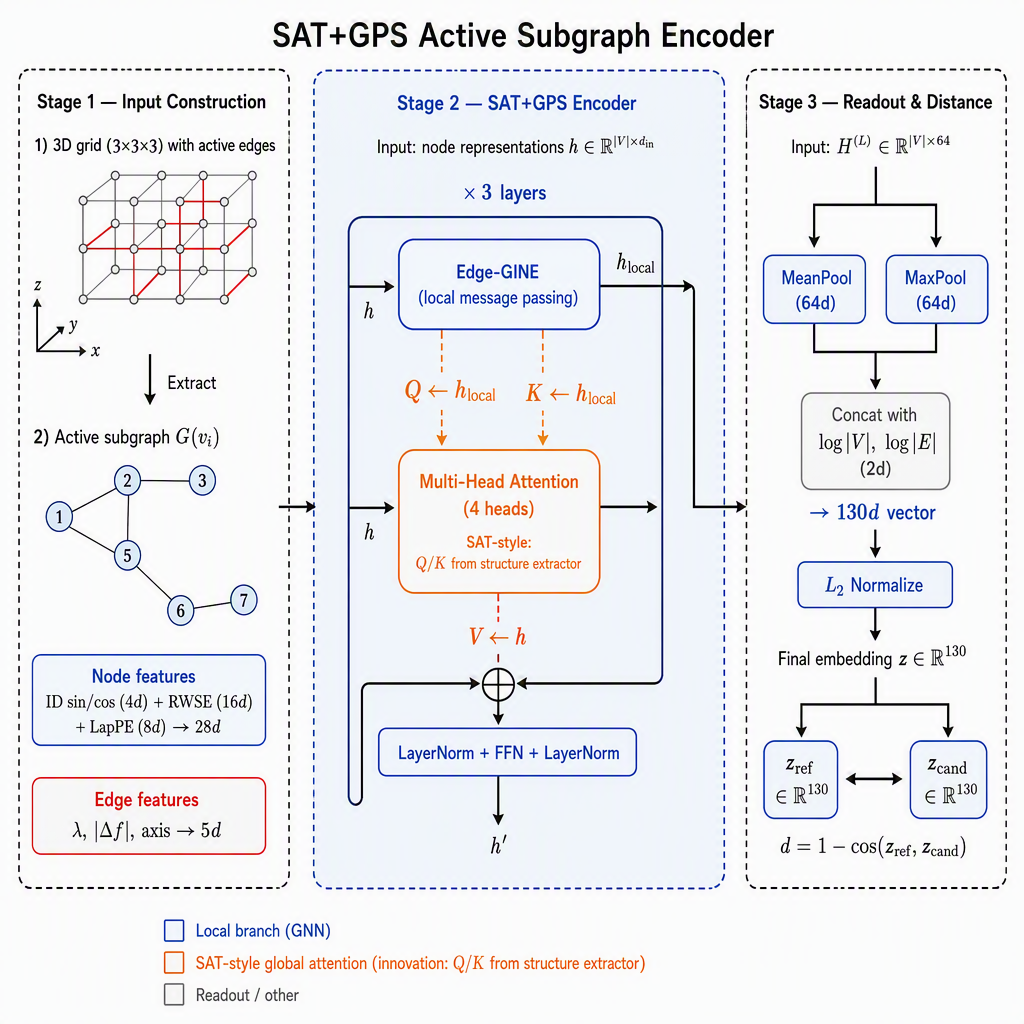
\includegraphics[width=0.9\linewidth]{GNN.jpeg}
\caption{基于 SAT+GPS 的活性子图结构编码器架构。左：从三维网格提取活性子图并构造节点/边特征；中：3 层 SAT+GPS Block（局部 Edge-GINE 与 SAT 风格全局注意力，Q/K 取自局部输出 $h_{\mathrm{local}}$）；右：双池化读出与余弦距离计算。}
\label{fig:gnn-pipeline}
\end{figure}

\paragraph{编码器输入图构造。}给定分段线性标量场 $f$ 及其轮廓树 $\mathcal{T}$，为分支 $b_\ell$ 上的候选节点 $v_i$ 构造编码器输入图的完整步骤如下。

记底层网格为 $\Omega=(V_\Omega, E_\Omega)$：$V_\Omega$ 为三维空间中的规则采样点，每个顶点 $p$ 携带坐标 $\mathrm{pos}(p)\in\mathbb{R}^3$ 与标量值 $f(p)\in\mathbb{R}$；$E_\Omega$ 连接空间相邻的顶点对。标量场沿每条边线性插值：
\begin{equation}
f\bigl((1{-}\lambda)p+\lambda q\bigr)=(1{-}\lambda)\,f(p)+\lambda\,f(q),\quad \lambda\in[0,1].
\label{eq:pl-interp}
\end{equation}

\noindent\textbf{步骤 1：确定阈值。}轮廓树 $\mathcal{T}$ 的每条分支 $b_\ell$ 连接两个关键点，索引了一组拓扑类型相同的等值面。对分支 $b_\ell$ 上的节点 $v_i$，取阈值 $t=f(v_i)$。

\noindent\textbf{步骤 2：提取活性边集合（边定义）。}遍历网格边集 $E_\Omega$，收集所有两端标量值跨越阈值 $t$ 的边，构成活性边集合：
\begin{equation}
E_{\mathrm{act}}(v_i)=\bigl\{(p,q)\in E_\Omega \;\big|\; \bigl(f(p)-t\bigr)\bigl(f(q)-t\bigr)<0 \bigr\}.
\label{eq:active-edges}
\end{equation}
每条活性边对应阈值 $t$ 的等值面穿过的一个网格单元边界——等值面的一个插值点恰好位于该边上。

\noindent\textbf{步骤 3：收集活性顶点集合（顶点定义）。}取所有活性边端点的并集作为顶点集：
\begin{equation}
V_{\mathrm{act}}(v_i)=\bigl\{p\in V_\Omega \;\big|\; \exists\, q:\,(p,q)\in E_{\mathrm{act}}(v_i)\bigr\}.
\label{eq:active-verts}
\end{equation}
每个活性顶点是原网格中紧邻等值面的采样点，继承其空间坐标 $\mathrm{pos}(p)$ 与标量值 $f(p)$。

\noindent\textbf{步骤 4：构成输入图。}以上述 $V_{\mathrm{act}}$ 为顶点集、$E_{\mathrm{act}}$ 为边集，构成无向图 $G_\ell(v_i)=(V_{\mathrm{act}}, E_{\mathrm{act}})$ 作为编码器的输入。图中顶点间的邻接关系直接继承自原网格 $\Omega$ 的空间邻接——即两个活性顶点之间存在边当且仅当它们在原网格中相邻且该边为活性边。

这样构造的输入图具有明确的物理语义：顶点是等值面附近的场采样点，边是等值面穿过的网格单元边界，图的连通结构直接反映了分支 $b_\ell$ 在阈值 $t$ 处等值面的空间形态与拓扑。不同阈值产生不同的活性子图，同一分支内等值面的几何演化即体现为活性子图的结构变化。

\paragraph{节点特征与位置编码。}对每个活性顶点 $p$，基础特征为 4 维 ID 正余弦位置编码：以顶点在原网格中的线性编号 $\mathrm{id}(p)$ 为输入，经两组不同周期的正余弦变换得到
\[
x^{\mathrm{ID}}_p = \bigl[\sin(\mathrm{id}/P_1),\;\cos(\mathrm{id}/P_1),\;\sin(\mathrm{id}/P_2),\;\cos(\mathrm{id}/P_2)\bigr],
\]
其中 $P_1{=}17,\;P_2{=}53$ 为预设周期。在此基础上，为每个活性子图拼接两类结构编码：16 维随机游走结构编码（RWSE）\cite{dwivedi_rwse_2022} 捕捉顶点在图中的局部可达性，8 维拉普拉斯位置编码（LapPE）\cite{dwivedi_benchmarking_2020} 捕捉全局谱结构。三者拼接得 $28$ 维特征，构成特征矩阵 $X\in\mathbb{R}^{|V_{\mathrm{act}}|\times 28}$。

\paragraph{边特征。}活性子图的每条有向边 $p\to q$ 携带 5 维属性向量。第一维为等值面在该边上的线性插值位置
\begin{equation}
\lambda_{p\to q} = \mathrm{clamp}\!\Bigl(\frac{t - f(p)}{f(q) - f(p)},\;0,\;1\Bigr),
\label{eq:lambda-edge}
\end{equation}
提供 Jaccard 二值边集所不具备的连续几何信息；反向边使用 $1{-}\lambda$。第二维为标量差绝对值 $|f(q){-}f(p)|$，后三维为网格轴向 one-hot 编码 $(\mathbf{e}_x,\mathbf{e}_y,\mathbf{e}_z)$，标识该边在规则网格中的方向。五维属性共同刻画等值面穿越每条网格边的方式与位置。

\paragraph{SAT+GPS 编码器。}以 $X$ 和活性子图邻接及边属性为输入，采用 3 层 SATGraphGPS 编码器。每层由两个并行分支组成：局部分支为带边属性的 Edge-GINE\cite{xu_gin_2019} 消息传递，全局分支为 4 头 Structure-Aware Transformer 注意力。\cite{chen_sat_2022} 具体地，第 $l$ 层的更新为
\begin{align}
h^{(l)}_{\mathrm{local}} &= \operatorname{Edge\text{-}GINE}\bigl(H^{(l-1)},\, E_{\mathrm{attr}}\bigr), \label{eq:edgegine}\\
h^{(l)}_{\mathrm{global}} &= \operatorname{MHA}\bigl(h^{(l)}_{\mathrm{local}},\, h^{(l)}_{\mathrm{local}},\, H^{(l-1)}\bigr), \label{eq:sat-attn}\\
H^{(l)} &= \operatorname{FFN}\bigl(\operatorname{LN}(H^{(l-1)}{+}h^{(l)}_{\mathrm{local}}) + \operatorname{LN}(H^{(l-1)}{+}h^{(l)}_{\mathrm{global}})\bigr), \nonumber
\end{align}
其中 $H^{(0)}{=}X$，$E_{\mathrm{attr}}$ 为 5 维边属性矩阵。SAT 风格注意力的关键在于式~\eqref{eq:sat-attn}：query 和 key 均来自局部消息传递的输出 $h_{\mathrm{local}}$，而 value 取原始节点状态 $H^{(l-1)}$——这使局部结构提取器控制全局注意力中的匹配模式，同时保留未经局部聚合的原始信息作为传递内容。\cite{rampasek_gps_2022} 隐藏维度 $h{=}64$，3 层聚合使每个顶点表示融合多跳邻域与全局上下文。

\paragraph{自监督训练。}编码器通过 NT-Xent\cite{chen_simclr_2020} 对比学习目标训练：正样本对由同一轮廓树分支上相邻的普通节点构成，或由同一节点对应的轻微标量扰动（$\delta{=}0.01$）副本构成；其余图对视为负样本。训练数据来自 20 个合成数据集中的 14 个（验证集为 case09、case13、case18，测试集为 case01、case17、case20），共约 6{,}383 个正样本对。优化器为 AdamW（学习率 $5{\times}10^{-4}$，权重衰减 $10^{-4}$），批量大小 16，温度参数 $\tau{=}0.1$，dropout 比率 $0.1$。训练对 LapPE 随机进行符号翻转，以处理拉普拉斯特征向量的符号不确定性。模型参数量约 200K。

随后从变长的顶点表示 $\{h^{(L)}_p\}$ 读出定长图级向量，采用双池化加规模编码：
\begin{multline}
z_\ell(v)=\mathrm{L2Norm}\bigl[\operatorname{MeanPool}(H^{(L)})\;\|\;\operatorname{MaxPool}(H^{(L)})\\
\;\|\;\log(1{+}|V_{\mathrm{act}}|)\;\|\;\log(1{+}|E_{\mathrm{act}}|)\bigr],
\label{eq:readout}
\end{multline}
其中 $\|$ 为向量拼接，$L{=}3$ 为层数。均值池化（$64$ 维）反映全局结构趋势，最大值池化（$64$ 维）捕捉最显著的局部特征；两个对数规模项弥补池化丢失的规模信息，使结构相似但规模不同的等值面仍可区分。经 $L_2$ 归一化映射到单位超球面，得 $z_\ell(v)\in\mathbb{R}^{130}$。

\paragraph{差异计算。}SAT+GPS 编码器输出的余弦距离为
\begin{equation}
d^{\mathrm{cos}}_\ell(v_r,v_i)=1-\cos\bigl(z_\ell(v_r),\,z_\ell(v_i)\bigr).
\label{eq:gnndist}
\end{equation}
由于 $z_\ell$ 已经 $L_2$ 归一化，$d^{\mathrm{cos}}_\ell{=}0$ 意味着两个活性子图的编码完全对齐，$d^{\mathrm{cos}}_\ell{=}2$ 为理论最大值。

为进一步利用活性边上的连续几何信息，引入\textbf{$\lambda$ 对齐残差}。对参考节点 $v_r$ 与候选节点 $v_i$ 的共同活性边集合 $E_{\cap}=E_{\mathrm{act}}(v_r)\cap E_{\mathrm{act}}(v_i)$，每条边上的插值位置差衡量等值面在相同网格边上的位移量：
\begin{equation}
R_\lambda(v_r,v_i) = \frac{1}{|E_\cap|}\sum_{e\in E_\cap}\bigl|\lambda_r(e)-\lambda_i(e)\bigr|,
\label{eq:lambda-residual}
\end{equation}
其中 $\lambda_r(e)$ 和 $\lambda_i(e)$ 分别为参考节点和候选节点阈值下边 $e$ 的线性插值位置（式~\eqref{eq:lambda-edge}）。$R_\lambda$ 捕捉了 Jaccard 二值边集无法区分的微细位移——两个阈值可能穿过完全相同的网格边（$d^J{=}0$），但等值面在这些边上的精确位置已经发生偏移。

三者加权组合为最终的分支差异度量：
\begin{equation}
d_\ell(v_r,v_i)=w_g\,d^{\mathrm{cos}}_\ell + (1{-}w_g)\,\bigl(d^J_\ell + w_\lambda\,R_\lambda\bigr),
\label{eq:pair-dist}
\end{equation}
其中 $w_g\in[0,1]$ 控制 SAT+GPS 编码距离的权重，$w_\lambda$ 控制 $\lambda$ 残差相对于 Jaccard 的灵敏度。$w_g{=}0$ 退化为纯 Jaccard 加 $\lambda$ 残差的基线；$w_g{=}1$ 退化为纯余弦距离——但如 \ref{sec:exp-weight-sweep} 节所示，纯余弦距离目前不够稳定，中等权重 $w_g{=}0.20$ 为推荐配置（$w_\lambda{=}0.25$）。

% ========================================
% 3.4 基于多分支加权的贪心简化算法
% ========================================
\subsection{基于多分支加权的贪心简化算法}
\label{sec:greedy}

基于前述多分支权重（\ref{sec:branch-weight} 节）、亏格不变约束（\ref{sec:genus-interval} 节）和分支几何差异（\ref{sec:geo-repr} 节），本节给出完整的贪心简化算法。

给定增广轮廓树 $T=(V,E,f)$ 和容差 $\varepsilon>0$，目标是寻找保留集合 $K\subseteq V$，使 $V_s\subseteq K$（结构节点全部保留），且在每条分支 $b=(v_0,\ldots,v_k)$ 内，相邻保留节点之间的多分支加权差异满足 $D(u_{j-1},u_j)<\varepsilon$。算法对每条分支独立执行链上贪心：保留起点 $v_0$ 并令 $v_r\leftarrow v_0$，依次扫描中间候选节点 $v_i$，计算活跃分支集合 $\mathcal{B}(t_i)$ 上的加权差异 $D(v_r,v_i)$（式~\eqref{eq:aggregate}）；若 $D\geq\varepsilon$ 则保留 $v_i$ 并更新参考节点，否则跳过；扫描结束后始终保留终点 $v_k$。

\begin{algorithm}[H]
\caption{基于多分支加权的贪心简化}
\label{alg:framework}
\begin{algorithmic}[1]
\Require 增广轮廓树 $T=(V,E,f)$，容差 $\varepsilon$，混合系数 $\alpha$，SAT 权重 $w_g$，$\lambda$ 权重 $w_\lambda$
\Ensure 保留节点集合 $K$，几何过滤增广轮廓树 $T'$
\State 识别结构节点 $V_s$，分解拓扑分支 $\{b_1,\ldots,b_n\}$
\State $K \gets V_s$
\ForAll{拓扑分支 $b=(v_0,\ldots,v_k)$}
  \State $v_r \gets v_0$
  \For{$i \gets 1$ \textbf{to} $k-1$}
    \State $t_i \gets f(v_i)$
    \State $\mathcal{B}(t_i) \gets$ 式~\eqref{eq:active-branch} 确定的活跃分支集合
    \ForAll{$b_\ell \in \mathcal{B}(t_i)$}
      \State $d_\ell \gets \textsc{BranchDiff}(v_r,v_i,b_\ell)$ \Comment{式~\eqref{eq:pair-dist}}
      \State 由式~\eqref{eq:weights}、\eqref{eq:wmix} 计算 $w_\ell$
    \EndFor
    \State $D \gets \sum_\ell w_\ell\, d_\ell$
    \If{$D \ge \varepsilon$}
      \State $K \gets K \cup \{v_i\}$；$v_r \gets v_i$
    \EndIf
  \EndFor
\EndFor
\State 合并被删节点跨越的弧，重建 $T'$
\State \Return $K,\ T'$
\end{algorithmic}
\end{algorithm}

全部分支完成保留判定后，合并被删节点跨越的弧（新弧标量跨度取两端保留节点之差、区域规模取被合并各弧之和），重建得到的 $T'$ 保持原树根、叶和分支节点结构，是一棵合法的几何过滤增广轮廓树。

\paragraph{复杂度。}结构节点识别与分支分解为 $O(|V|)$。链上贪心对每个候选节点各处理一次，在至多 $q$ 个活跃分支上计算差异，总代价为 $O(|V_o|\,q\,C(\bar{s}))$，其中 $C(\bar{s})$ 为单分支差异代价：Jaccard 与 $\lambda$ 残差为 $O(\bar{s})$（边集交并与插值位置差），SAT+GPS 为 $O(\bar{s}\,h\,L)$（$L{=}3$ 层前向传播），$\bar{s}$ 为平均活性边数、$h{=}64$ 为隐藏维度。参考节点的 embedding 可缓存，避免重复计算。

\section{实验}
\label{sec:experiments}

本节实验组织如下：\ref{sec:exp-topo} 节验证拓扑正确性与 $\varepsilon$ 的单调控制；\ref{sec:exp-geom} 节以 Jaccard 为基线对比 SAT+GPS 增强度量的几何代表性——这是本文的核心实验；\ref{sec:exp-weight-sweep} 节分析 SAT 权重的影响；\ref{sec:exp-test-subset} 节报告测试子集结果；\ref{sec:exp-multibranch} 节分析多分支加权的作用与适用条件；\ref{sec:exp-vis} 与 \ref{sec:exp-discussion} 节给出可视化与综合讨论。

\subsection{实验设置与数据集}
\label{sec:exp-setup}

实验在配备 NVIDIA GeForce RTX 3080 Ti（12\,GB 显存）的工作站上运行，使用 Topology ToolKit（TTK）提取增广轮廓树，C++ 实现基于 VTK 9.6，SAT+GPS 编码器及简化器基于 PyTorch 2.1。编码器超参数如 \ref{sec:gnn} 节所述（$h{=}64$，$L{=}3$，4 头注意力，约 200K 参数），训练采用 AdamW（$\mathrm{lr}{=}5{\times}10^{-4}$，权重衰减 $10^{-4}$），批量大小 16，温度 $\tau{=}0.1$，固定随机种子保证可复现。除特别说明外，默认参数为混合系数 $\alpha = 0.40$，SAT 权重 $w_g = 0.20$，$\lambda$ 权重 $w_\lambda = 0.25$。

数据集为 20 个规则网格上的合成标量场（case01--case20，网格规模 $5\times5\times3$ 至 $12\times8\times5$，树节点数 75--500，分支数 7--44），增广轮廓树由 TTK 的 FTM 算法提取。SAT+GPS 编码器在其中 14 个 case 上训练，case09、case13、case18 为验证集，case01、case17、case20 为测试集（未参与编码器训练）。主结果在全部 20 个数据集上报告，并单独给出测试子集结果以评估泛化性（\ref{sec:exp-test-subset} 节）。各方法在每个 case 上单独校准容差 $\varepsilon$ 使保留节点数对齐到约 50\%，保证公平比较。
\label{sec:exp-dataset}

\subsection{评估指标}
\label{sec:exp-metrics}

拓扑正确性与简化强度分别由\textbf{结构节点保留率} $R_s = |V_s \cap K| / |V_s|$（本文方法设计上应恒为 100\%）与\textbf{节点压缩率} $C = (|V| - |K|)/|V|$ 刻画。几何代表性需要多视角评估——单一距离既容易与筛选度量同源、无法公平对比，也难以同时反映"逐点几何"与"整体属性"两个层面。为此从两条互补主线组织指标：\textbf{近邻近似误差}继承 Metro 框架\cite{cignoni_metro_1998,livesu_mesh_quality_2023}，\textbf{属性曲线误差}继承等值面谱与 key-isovalue 信息损失曲线\cite{bajaj_spectrum_1997,zhou_keyisovalue_2025}。

\paragraph{近邻近似误差（NNAE）。}量化"被删除节点是否被相邻保留节点良好代表"：对每个被删节点 $v_d \in V \setminus K$，在 $K$ 中取标量值最近邻 $v_k^*$，以几何距离 $d(\cdot,\cdot)$ 衡量二者的等值面差异后求均值：
\begin{equation}
\text{NNAE}^{d} = \frac{1}{|V \setminus K|}\sum_{v_d \in V\setminus K} d(v_d, v_k^*).
\end{equation}
$d$ 取三种实例：\textbf{对称 Hausdorff 距离}（NNAE$^H$，最坏情况偏差）、\textbf{对称 Chamfer 距离}（NNAE$^C$，对离群点更鲁棒，近年 3D 表面重建的默认指标）、\textbf{活性边 Jaccard 距离}（NNAE$^J$，方法内部一致性参考）。前两者通过 Marching Cubes\cite{lorensen_cline_1987} 显式重建 $v_d$ 与 $v_k^*$ 的等值面网格后计算、按包围盒对角线归一化，与本文任何筛选度量相互独立，是\textbf{中立的第三方指标}。另报告 p90 分位数衡量尾部最差情况。

\paragraph{属性曲线误差（PCE）。}从互补角度刻画简化前后\textbf{整体属性}的对齐性：分别在 $V$ 与 $K$ 上计算每个节点等值面的面积 $A(t)$ 与体积 $V(t)$ 曲线，用保留节点分段线性插值后与原始曲线做相对 $L_2$ 误差，记 $\text{PCE}_A$ 与 $\text{PCE}_V$。PCE 越小说明保留节点可以准确重建原始属性演化。

\paragraph{分支保留率分布。}每条分支 $b_\ell$ 上保留节点占比 $|K \cap b_\ell| / |b_\ell|$ 的分布，用于检验是否存在分支被过度简化。

\subsection{拓扑正确性与压缩率控制}
\label{sec:exp-topo}

\paragraph{拓扑正确性。}对全部 20 个数据集，在 $\varepsilon \in \{0.1, 0.3, 0.5, 0.7\}$ 下运行本文方法（Jaccard 配置），所有 80 组运行的结构节点保留率均为 $R_s = 100\%$——结构节点的无条件保留是算法的硬约束（算法~\ref{alg:framework} 第 2 行），与 $\varepsilon$ 取值无关，\ref{sec:genus-interval} 节"不丢失任何连通性与亏格变化事件"的声明由此得证。
\label{sec:exp-param}

\paragraph{$\varepsilon$ 单调控制。}固定 $\alpha = 0.40$ 扫描 $\varepsilon \in [0.05, 0.80]$，压缩率 $C$ 随 $\varepsilon$ 严格单调不减（图~\ref{fig:eps-sweep}），用户可通过单一参数连续控制简化强度。

\begin{figure}[h]
\centering
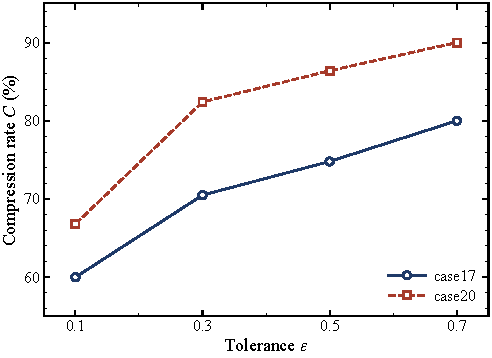
\includegraphics[width=0.9\linewidth]{fig-eps-sweep.pdf}
\caption{容差 $\varepsilon$ 对压缩率 $C$ 的单调控制。case17（实线）与 case20（虚线）上，$C$ 随 $\varepsilon$ 严格单调不减；$\varepsilon\in[0.3,0.5]$ 为推荐工作区间。}
\label{fig:eps-sweep}
\end{figure}

\subsection{SAT+GPS 增强的几何差异度量}
\label{sec:exp-geom}

本节验证本文的核心方法贡献：\textbf{SAT+GPS 结构表示与 $\lambda$ 连续边信息结合后，能在相同压缩率下改善纯 Jaccard 基线的几何代表性}。所有方法均以多分支加权配置运行（$\alpha{=}0.40$），对每个 case 单独校准 $\varepsilon$ 使保留节点数对齐到约 50\%；NNAE$^{C/H}$ 已按包围盒对角线归一化，与本文任何筛选度量相互独立。

\begin{table}[t]
\centering
\scriptsize
\caption{20-case 平均结果（multi 配置，压缩率 $\approx 50\%$）。SAT+GPS pairrisk 配置：$w_g{=}0.20$，$w_\lambda{=}0.25$。\textbf{加粗}为该列最优。}
\label{tab:geom-comparison}
\begin{tabular}{@{}lrrr@{\hspace{8pt}}rr@{}}
\hline
方法 & NNAE$^C$ & NNAE$^H$ & NNAE$^J$ & PCE$_A$ & PCE$_V$ \\
\hline
Jaccard-multi & 0.00259 & 0.03030 & 0.05382 & 0.00497 & 0.02455 \\
SAT+GPS       & \textbf{0.00246} & \textbf{0.02900} & \textbf{0.05286} & \textbf{0.00477} & \textbf{0.02443} \\
\hline
相对变化 & $-4.84\%$ & $-4.28\%$ & $-1.79\%$ & $-4.19\%$ & $-0.52\%$ \\
\hline
\end{tabular}
\end{table}

结果如表~\ref{tab:geom-comparison} 所示。\textbf{在全部 5 类指标下，SAT+GPS 增强的 pair-aligned 度量均优于纯 Jaccard 基线}：NNAE$^C$（Chamfer 距离）下降 $4.84\%$，NNAE$^H$（Hausdorff 距离）下降 $4.28\%$，PCE$_A$（面积属性误差）下降 $4.19\%$。逐 case 统计中，SAT+GPS 分别在 15/20、14/20、15/20、13/20、12/20 个 case 上优于 Jaccard，说明改善具有多数覆盖性而非个别 case 驱动。

需要强调的是，当前结果是 SAT+GPS 编码距离、Jaccard 距离与 $\lambda$ 对齐残差的混合方法（式~\eqref{eq:pair-dist}），SAT+GPS 余弦距离在推荐配置中仅占 $20\%$ 权重。纯余弦距离（$w_g{=}1.0$）目前明显不稳定（见 \ref{sec:exp-weight-sweep} 节），因此该结果不应解释为纯 SAT+GPS 已全面取代 Jaccard，而是三个信号源的协同改善。

\subsection{SAT 权重扫描}
\label{sec:exp-weight-sweep}

为考察 SAT+GPS 编码距离在最终混合距离（式~\eqref{eq:pair-dist}）中的最佳占比，固定 $w_\lambda{=}0.25$，在全部 20 个 case 上扫描 $w_g \in \{0.05, 0.10, 0.20, 0.35, 0.50, 0.75, 1.0\}$，每个配置单独校准 $\varepsilon$ 至约 50\% kept。表~\ref{tab:weight-sweep} 报告相对 Jaccard-multi 基线的五项平均误差变化。

\begin{table}[h]
\centering
\scriptsize
\caption{$w_g$ 扫描：相对 Jaccard-multi 的五项平均误差变化（$w_\lambda{=}0.25$，20-case 平均，$\approx 50\%$ kept）。负值表示改善。}
\label{tab:weight-sweep}
\begin{tabular}{@{}rrrrrr@{}}
\hline
$w_g$ & $\Delta$NNAE$^C$ & $\Delta$NNAE$^H$ & $\Delta$NNAE$^J$ & $\Delta$PCE$_A$ & $\Delta$PCE$_V$ \\
\hline
0.05 & $-2.0\%$ & $-2.0\%$ & $-1.3\%$ & $-2.3\%$ & $-0.8\%$ \\
0.10 & $-3.2\%$ & $-3.7\%$ & $-1.7\%$ & $-1.3\%$ & $-0.3\%$ \\
\textbf{0.20} & $\mathbf{-4.8\%}$ & $\mathbf{-4.3\%}$ & $\mathbf{-1.8\%}$ & $\mathbf{-4.2\%}$ & $\mathbf{-0.5\%}$ \\
0.35 & $-5.9\%$ & $-5.8\%$ & $-1.3\%$ & $-2.4\%$ & $-0.1\%$ \\
0.50 & $-5.4\%$ & $-4.2\%$ & $+1.8\%$ & $+0.6\%$ & $+0.7\%$ \\
0.75 & $-0.2\%$ & $-1.0\%$ & $+4.4\%$ & $-0.8\%$ & $+6.9\%$ \\
1.00 & $+36.6\%$ & $+22.8\%$ & $+29.8\%$ & $+20.0\%$ & $+29.2\%$ \\
\hline
\end{tabular}
\end{table}

$w_g{\leq}0.35$ 时五项指标均改善或基本持平；$w_g{=}0.20$ 在 Chamfer、Hausdorff 和面积属性三个维度上取得最均衡的改善，为推荐配置。$w_g{\geq}0.50$ 后 NNAE$^J$ 和 PCE 开始退化，$w_g{=}1.0$（纯余弦距离）五项指标全面恶化——这是因为 NT-Xent 训练目标保证了相邻节点在表示空间中的相对距离，但并未保证余弦距离与 Chamfer/Hausdorff/属性误差单调对应；此外，cosine 与 Jaccard 的数值尺度不同，未经校准时直接让 cosine 主导会造成距离尺度失配。中等权重让 SAT+GPS 提供结构感知的"微调"信号，同时保留 Jaccard 和 $\lambda$ 残差的稳定基底。

\subsection{测试子集结果}
\label{sec:exp-test-subset}

为评估 SAT+GPS 编码器在未参与训练的数据上的泛化性，表~\ref{tab:test-subset} 单独报告测试子集（case01、case17、case20）的结果。

\begin{table}[h]
\centering
\scriptsize
\caption{测试子集（case01/17/20，未参与编码器训练）的对比。}
\label{tab:test-subset}
\begin{tabular}{@{}lrrrrr@{}}
\hline
方法 & NNAE$^C$ & NNAE$^H$ & NNAE$^J$ & PCE$_A$ & PCE$_V$ \\
\hline
Jaccard-multi        & 0.00385 & 0.03522 & 0.06925 & 0.00874 & 0.02261 \\
SAT+GPS ($w_g{=}0.20$) & \textbf{0.00345} & \textbf{0.03253} & 0.07017 & \textbf{0.00800} & 0.02502 \\
\hline
\end{tabular}
\end{table}

测试子集上，SAT+GPS 的 Chamfer 距离降低 $10.2\%$，Hausdorff 距离降低 $7.6\%$，面积属性误差降低 $8.4\%$——改善幅度大于 20-case 全量平均，表明编码器在未见数据上的泛化良好。但 NNAE$^J$ 略高（$+1.3\%$）且 PCE$_V$ 略高（$+10.7\%$），说明在个别测试 case 上 SAT+GPS 对体积属性的保持不如 Jaccard 稳定。总体而言，在最重要的中立几何指标（Chamfer 和 Hausdorff）上，测试子集的结论与全量结果一致。

\subsection{多分支加权分析}
\label{sec:exp-multibranch}

本节独立分析多分支加权组件（\ref{sec:branch-weight} 节）的作用，从三个维度考察：整体几何代表性、分支覆盖均匀性、以及适用条件。

\paragraph{整体几何代表性。}表~\ref{tab:multi-vs-single} 报告 case17 与 case20 在 Jaccard 度量下 single 与 multi 配置的多视角对比（等压缩率）。case17 上 multi 在所有中立指标下（NNAE$^C$、NNAE$^H$、PCE$_A$/PCE$_V$）均一致优于 single：NNAE$^C$ 从 0.00105 降至 0.00088（-16\%），PCE$_A$ 从 0.0019 降至 0.0014（-26\%）；case20 上 multi 与 single 在中立指标下基本持平，说明 multi 对整体误差的贡献是数据依赖的。

\begin{table}[h]
\centering
\scriptsize
\caption{single vs multi 多视角对比（Jaccard 度量，$\alpha=0.40$，等压缩率）。}
\label{tab:multi-vs-single}
\begin{tabular}{lcccc}
\hline
配置 & 保留 & NNAE$^C$ & NNAE$^H$ & PCE$_A$ \\
\hline
\multicolumn{5}{l}{\textbf{case17（压缩率 $\approx 48\%$）}} \\
Jaccard-single & 192 & 0.00105 & 0.01932 & 0.0019 \\
Jaccard-multi  & 220 & \textbf{0.00088} & \textbf{0.01817} & \textbf{0.0014} \\
\hline
\multicolumn{5}{l}{\textbf{case20（压缩率 $\approx 55\%$）}} \\
Jaccard-single & 229 & \textbf{0.00076} & \textbf{0.01604} & \textbf{0.0014} \\
Jaccard-multi  & 227 & \textbf{0.00076} & 0.01601 & 0.0015 \\
\hline
\end{tabular}
\end{table}

\paragraph{分支覆盖均匀性。}上表反映的是整体误差，无法揭示节点在各分支间是否分配均衡。表~\ref{tab:branch-coverage} 报告每条分支保留率的分布统计——最小分支保留率 $r_{\min}$ 与均值 $\bar{r}$。$r_{\min}$ 的意义大于 $\bar{r}$：若某条分支保留率过低，意味着该分支上的几何演化关键节点被过度删除。多分支加权在 case17 上使 Jaccard 的 $r_{\min}$ 从 0.056 提高至 0.062（+11\%），SAT+GPS 的 $r_{\min}$ 从 0.050 提高至 0.059（+18\%）；对 case20，Jaccard 的 $r_{\min}$ 略降（0.343→0.339），SAT+GPS 的 $r_{\min}$ 提高（0.229→0.245）。整体上，多分支加权略微牺牲了 case17 的平均保留率 $\bar{r}$ 而换取了更均匀的分支覆盖。

\begin{table}[h]
\centering
\small
\caption{分支保留率分布（$\varepsilon$ 已调至同压缩率）。$r_{\min}$：最小分支保留率；$\bar{r}$：平均。}
\label{tab:branch-coverage}
\begin{tabular}{lcccc}
\hline
\multirow{2}{*}{配置} & \multicolumn{2}{c}{case17} & \multicolumn{2}{c}{case20} \\
                     & $r_{\min}$ & $\bar{r}$ & $r_{\min}$ & $\bar{r}$ \\
\hline
Jaccard-single    & 0.056 & \textbf{0.599} & \textbf{0.343} & 0.829 \\
Jaccard-multi     & \textbf{0.062} & 0.641 & 0.339 & \textbf{0.831} \\
SAT+GPS-single        & 0.050 & 0.517 & 0.229 & 0.778 \\
SAT+GPS-multi         & \textbf{0.059} & 0.585 & \textbf{0.245} & \textbf{0.799} \\
\hline
\end{tabular}
\end{table}

\paragraph{适用条件分析（20 case 全量）。}case17 与 case20 上 multi 的结论看似矛盾（一个受益、一个几乎无差异），提示多分支加权的增益依赖于数据本身的分支结构。为定量刻画这一依赖，我们在全部 20 个合成数据集上，对每个数据集分别为 single 与 multi 二分调 $\varepsilon$ 至同压缩率（目标 50\%），统计 multi 相对 single 的 NNAE$^J$ 相对增益 $\Delta = (E_s - E_m) / E_s$。为刻画数据的"分支重叠程度"，定义\textbf{平均活跃分支数}
\begin{equation}
\bar{q} = \frac{1}{|V_o|} \sum_{v_i \in V_o} |\mathcal{B}(t_i)|,
\label{eq:qbar}
\end{equation}
即所有普通节点标量层级上活跃分支数的均值。$\bar{q}$ 越大表示同一层级下同时活动的分支越多，$\bar{q}=1$ 表示每个层级仅有一条分支活跃、multi 退化为 single。

\begin{figure}[h]
\centering
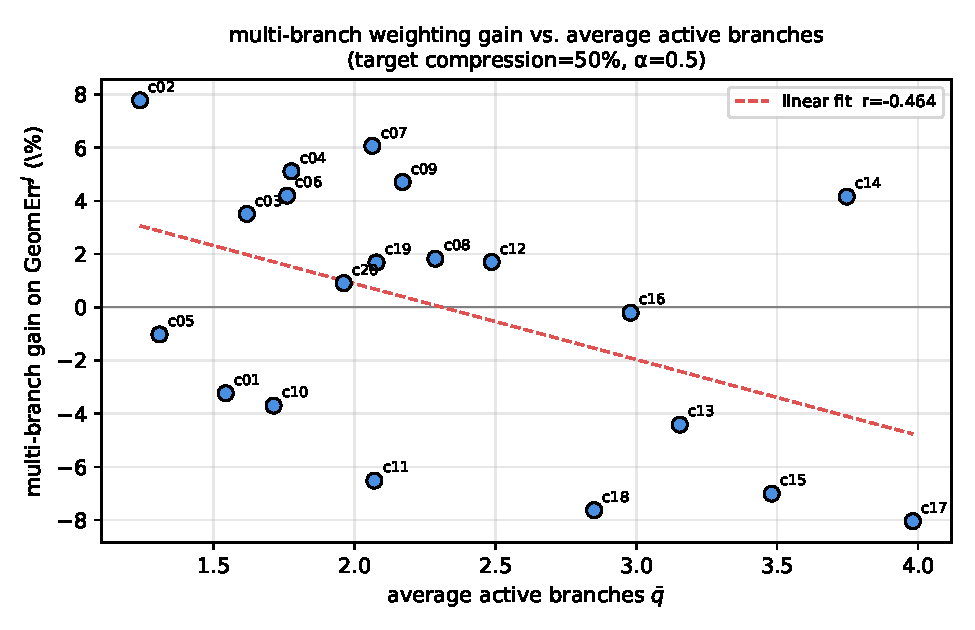
\includegraphics[width=0.95\linewidth]{fig-qbar-gain.pdf}
\caption{20 个合成数据集上 multi 相对 single 的 NNAE$^J$ 相对增益 $\Delta$ 与平均活跃分支数 $\bar{q}$ 的关系（等压缩率 50\%，$\alpha=0.40$，Jaccard 度量）。虚线为线性拟合，Pearson $r=-0.46$。$\bar{q}$ 较小时 multi 更常有正增益；$\bar{q}$ 较大时正负相抵，均值接近 0。}
\label{fig:qbar-gain}
\end{figure}

图~\ref{fig:qbar-gain} 显示，$\bar{q}$ 与 $\Delta$ 呈弱负相关（Pearson $r=-0.46$）；20 case 上 $\Delta$ 均值 $-0.01\%$、中位数 $+1.29\%$，11/20 为正。这说明\textbf{多分支加权对整体几何代表性的贡献是数据依赖的}：活跃分支较多时，加权平均反而会摊平不同分支的差异、稀释主链上的显著节点。结合表~\ref{tab:branch-coverage}，多分支加权的稳定价值在于\textbf{分支覆盖均匀性}（$r_{\min}$ 在多数配置下提升）——以可能牺牲少量整体误差为代价，换取每条分支"最坏情况"的改善。实用建议：存在语义关键的小分支必须保留时开启，追求整体误差最小时关闭。

\paragraph{$\alpha$ 参数敏感性。}固定 $\varepsilon = 0.4$，扫描 $\alpha \in \{0, 0.25, 0.5, 0.75, 1\}$（表~\ref{tab:alpha-sensitivity}）。总保留数变化在 10\% 以内，$r_{\min}$ 基本不变——说明多分支加权对拓扑权重与几何规模权重的具体比例不敏感，两种权重都能识别"重要分支"，只是排序略有差异。$\alpha=0.40$ 为推荐默认，同时兼顾持久性（$\alpha=1$）与当前几何规模变化（$\alpha=0$）信息。

\begin{table}[h]
\centering
\scriptsize
\caption{$\alpha$ 敏感性（$\varepsilon=0.4$，Jaccard-multi 配置）。}
\label{tab:alpha-sensitivity}
\begin{tabular}{lccccc}
\hline
$\alpha$   & 0 & 0.25 & 0.5 & 0.75 & 1 \\
\hline
case17 保留数   & 114 & 114 & 113 & 105 & 103 \\
case17 $r_{\min}$ & 0.062 & 0.062 & 0.052 & 0.052 & 0.052 \\
case20 保留数   & 77 & 77 & 75 & 75 & 74 \\
case20 $r_{\min}$ & 0.055 & 0.055 & 0.055 & 0.055 & 0.055 \\
\hline
\end{tabular}
\end{table}

\subsection{可视化结果}
\label{sec:exp-vis}

[\textit{占位段落，待补充可视化图片。}] 图~\ref{fig:vis-tree}（待补）展示 case01 上原始增广轮廓树与本文方法简化树的对比：结构节点以红色标注，保留的普通节点以蓝色标注，被删节点以浅灰标注。图~\ref{fig:vis-isosurface}（待补）展示 case17 数据集在 [\textit{$k$ 待定}] 个保留节点对应阈值下的等值面序列——这些等值面涵盖了不同拓扑层级下的等值结构演化，验证了保留节点的几何代表性。

\subsection{讨论与局限}
\label{sec:exp-discussion}

\paragraph{适用性总结。}SAT+GPS 增强的 pair-aligned 度量在全部 5 类评估指标下优于纯 Jaccard 基线（\ref{sec:exp-geom} 节），且在测试子集上泛化良好（\ref{sec:exp-test-subset} 节），适用于任何以增广轮廓树为骨架、需要在保持拓扑关键点的同时压缩节点冗余的场景。组件选择上：SAT 权重 $w_g{=}0.20$ 为综合最优，$w_g{\geq}0.50$ 后开始退化（\ref{sec:exp-weight-sweep} 节）；多分支加权的贡献是数据依赖的，其稳定价值在于分支覆盖均匀性——关心"每条分支的最坏情况"时开启，追求整体误差最小时关闭（\ref{sec:exp-multibranch} 节）。

\paragraph{当前局限。}（1）实验数据规模较小（最大 $12\times 8\times 5$）且均为规则合成网格，方法在大规模真实体数据（如医学 CT、湍流仿真）上的表现仍待验证——尤其是活性子图提取和 SAT+GPS 前向传播的时间/内存可扩展性。（2）极高压缩率（${>}80\%$）下，分支内节点分布可能不均——单条分支仅保留端点、丢失中间演化。（3）纯余弦距离（$w_g{=}1.0$）目前明显不稳定，说明 NT-Xent 训练目标与下游几何误差之间尚缺直接对齐；引入以 Chamfer/Hausdorff 误差为监督信号的几何风险头有望实现真正的纯 SAT+GPS 替代方案。（4）当前结果基于单一训练种子和单一约 50\% 压缩率，尚未报告多种子标准差和多压缩率的统计显著性验证。（5）运行时间与内存占用的系统性测量待补充（\textit{占位}）。

\clearpage
\begin{thebibliography}{99}

% === 背景 ===

\bibitem{lorensen_cline_1987}
W. E. Lorensen and H. E. Cline.
Marching cubes: A high resolution 3D surface construction algorithm.
\textit{Computer Graphics}, 21(4):163--169, 1987.

\bibitem{edelsbrunner_harer_2010}
H. Edelsbrunner and J. L. Harer.
\textit{Computational Topology: An Introduction}.
American Mathematical Society, 2010.

\bibitem{milnor_morse_1963}
J. Milnor.
\textit{Morse Theory}.
Princeton University Press, 1963.

\bibitem{ni_fair_2004}
X. Ni, M. Garland, and J. C. Hart.
Fair Morse functions for extracting the topological structure of a surface mesh.
\textit{ACM Transactions on Graphics}, 23(3):613--622, 2004.

% === 2.2.1 拓扑简化 ===

\bibitem{van_kreveld_1997}
M. van Kreveld, R. van Oostrum, C. Bajaj, V. Pascucci, and D. Schikore.
Contour trees and small seed sets for isosurface traversal.
\textit{Proceedings of the 13th Annual Symposium on Computational Geometry}, pages 212--220, 1997.

\bibitem{carr_contour_2003}
H. Carr, J. Snoeyink, and U. Axen.
Computing contour trees in all dimensions.
\textit{Computational Geometry}, 24(2):75--94, 2003.

\bibitem{edelsbrunner_persistence_2002}
H. Edelsbrunner, D. Letscher, and A. Zomorodian.
Topological persistence and simplification.
\textit{Discrete \& Computational Geometry}, 28(4):511--533, 2002.

\bibitem{carr_geometric_2004}
H. Carr, J. Snoeyink, and M. van de Panne.
Simplifying flexible isosurfaces using local geometric measures.
\textit{IEEE Visualization}, pages 497--504, 2004.

\bibitem{carr_flexible_2010}
H. Carr, J. Snoeyink, and M. van de Panne.
Flexible isosurfaces: Simplifying and displaying scalar topology using the contour tree.
\textit{Computational Geometry}, 43(1):42--58, 2010.

\bibitem{gueunet_act_2019}
C. Gueunet, P. Fortin, J. Jomier, and J. Tierny.
Task-based augmented contour trees with Fibonacci heaps.
\textit{IEEE Transactions on Parallel and Distributed Systems}, 30(8):1889--1905, 2019.

\bibitem{lukasczyk_extreem_2023}
J. Lukasczyk, M. Will, F. Wetzels, G. H. Weber, and C. Garth.
ExTreeM: Scalable augmented merge tree computation via extremum graphs.
\textit{IEEE Transactions on Visualization and Computer Graphics}, 2023.

\bibitem{tierny_ttk_2018}
J. Tierny, G. Favelier, J. A. Levine, C. Gueunet, and M. Michaux.
The Topology ToolKit.
\textit{IEEE Transactions on Visualization and Computer Graphics}, 24(1):832--842, 2018.

\bibitem{li_distributed_2024}
M. Li, H. Carr, O. R\"ubel, B. Wang, and G. H. Weber.
Distributed augmentation, hypersweeps, and branch decomposition of contour trees for scientific exploration.
\textit{IEEE Transactions on Visualization and Computer Graphics}, 2024.

\bibitem{li_presimplification_2025}
M. Li, H. Carr, O. R\"ubel, B. Wang, and G. H. Weber.
Extremely scalable distributed computation of contour trees via pre-simplification.
\textit{IEEE Symposium on Large Data Analysis and Visualization (LDAV)}, 2025.

\bibitem{sridharamurthy_local_2021}
R. Sridharamurthy and V. Natarajan.
Comparative analysis of merge trees using local tree edit distance.
\textit{IEEE Transactions on Visualization and Computer Graphics}, 29(2):1518--1530, 2023.

\bibitem{wetzels_path_2023}
F. Wetzels, M. Pont, J. Tierny, and C. Garth.
Merge tree geodesics and barycenters with path mappings.
\textit{IEEE Transactions on Visualization and Computer Graphics}, 2023.

\bibitem{pont_region_2025}
M. Pont and C. Garth.
Region-aware Wasserstein distances of persistence diagrams and merge trees.
\textit{IEEE Transactions on Visualization and Computer Graphics}, 2025.

% === 2.2.2 等值面几何简化 ===

\bibitem{cignoni_metro_1998}
P. Cignoni, C. Rocchini, and R. Scopigno.
Metro: Measuring error on simplified surfaces.
\textit{Computer Graphics Forum}, 17(2):167--174, 1998.

\bibitem{livesu_mesh_quality_2023}
M. Livesu, D. Pitzalis, and G. Cherchi.
A survey of indicators for mesh quality assessment.
\textit{Computer Graphics Forum} (Eurographics STAR), 42(2), 2023.

\bibitem{bajaj_spectrum_1997}
C. L. Bajaj, V. Pascucci, and D. R. Schikore.
The contour spectrum.
\textit{IEEE Visualization}, pages 167--174, 1997.

\bibitem{chiang_lu_2003}
Y.-J. Chiang and X. Lu.
Progressive simplification of tetrahedral meshes preserving all isosurface topologies.
\textit{Computer Graphics Forum}, 22(3):493--504, 2003.

\bibitem{bruckner_ism_2010}
S. Bruckner and T. M\"oller.
Isosurface similarity maps.
\textit{Computer Graphics Forum}, 29(3):773--782, 2010.

\bibitem{wang_isomeasure_2020}
Z. Wang.
Representative isovalue detection and isosurface segmentation using novel isosurface measures.
\textit{Computer Graphics Forum}, 39(3):37--47, 2020.

\bibitem{dai_isoexplorer_2021}
H. Dai, Y. Tao, X. He, and H. Lin.
IsoExplorer: An isosurface-driven framework for 3D shape analysis of biomedical volume data.
\textit{Journal of Visualization}, 2021.

\bibitem{he_scalargcn_2021}
X. He, Y. Tao, S. Yang, C. Chen, and H. Lin.
ScalarGCN: Scalar-value association analysis of volumes based on graph convolutional network.
\textit{Journal of Visualization}, 2021.

\bibitem{li_shen_inr_2024}
H. Li and H.-W. Shen.
Improving efficiency of iso-surface extraction on implicit neural representations using uncertainty propagation.
\textit{IEEE Transactions on Visualization and Computer Graphics}, 2024.

\bibitem{li_multiview_ism_2025}
P. Li, C. Chen, F. Wang, X. Zhang, and Y. Wang.
Multi-view isosurface similarity analysis for transfer function design in direct volume rendering.
\textit{Computers \& Graphics}, 2025.

\bibitem{zhou_keyisovalue_2025}
F. Zhou, H. Hu, F. Wang, J. Zhu, and W. Gao.
Key-isovalue selection and hierarchical exploration visualization of weather forecast ensembles.
\textit{Visual Informatics}, 2025.

% === 2.2.3 图表示学习 ===

\bibitem{kipf_gcn_2017}
T. N. Kipf and M. Welling.
Semi-supervised classification with graph convolutional networks.
\textit{International Conference on Learning Representations}, 2017.

\bibitem{gilmer_mpnn_2017}
J. Gilmer, S. S. Schoenholz, P. F. Riley, O. Vinyals, and G. E. Dahl.
Neural message passing for quantum chemistry.
\textit{International Conference on Machine Learning}, pages 1263--1272, 2017.

\bibitem{xu_gin_2019}
K. Xu, W. Hu, J. Leskovec, and S. Jegelka.
How powerful are graph neural networks?
\textit{International Conference on Learning Representations}, 2019.

\bibitem{rampasek_gps_2022}
L. Rampasek, M. Galkin, V. P. Dwivedi, A. T. Luu, G. Wolf, and D. Beaini.
Recipe for a general, powerful, scalable graph transformer.
\textit{Advances in Neural Information Processing Systems}, 35, 2022.

\bibitem{barshalom_subgraphormer_2024}
G. Bar-Shalom, B. Bevilacqua, and H. Maron.
Subgraphormer: Unifying subgraph GNNs and graph transformers via graph products.
\textit{International Conference on Machine Learning}, 2024.

\bibitem{hanocka_meshcnn_2019}
R. Hanocka, A. Hertz, N. Fish, R. Giryes, S. Fleishman, and D. Cohen-Or.
MeshCNN: A network with an edge.
\textit{ACM Transactions on Graphics}, 38(4):90:1--90:12, 2019.

\bibitem{sharp_diffusionnet_2022}
N. Sharp, S. Attaiki, K. Crane, and M. Ovsjanikov.
DiffusionNet: Discretization agnostic learning on surfaces.
\textit{ACM Transactions on Graphics}, 41(3):27:1--27:16, 2022.

\bibitem{jain_graphedx_2024}
E. Jain, I. Roy, S. Meher, S. Chakrabarti, and A. De.
Graph edit distance with general costs using neural set divergence.
\textit{Advances in Neural Information Processing Systems}, 37, 2024.

\bibitem{qin_mtnn_2024}
Y. Qin, B. T. Fasy, C. Wenk, and B. Summa.
Rapid and precise topological comparison with merge tree neural networks.
\textit{IEEE Transactions on Visualization and Computer Graphics}, 2024.

% === 本文新增引用 ===

\bibitem{ying_graphormer_2021}
C. Ying, T. Cai, S. Luo, S. Zheng, G. Ke, D. He, Y. Shen, and T.-Y. Liu.
Do transformers really perform bad for graph representation?
\textit{Advances in Neural Information Processing Systems}, 34, 2021.

\bibitem{kreuzer_san_2021}
D. Kreuzer, D. Beaini, W. L. Hamilton, V. L\'etourneau, and P. Tossou.
Rethinking graph transformers with spectral attention.
\textit{Advances in Neural Information Processing Systems}, 34, 2021.

\bibitem{lim_signnet_2023}
D. Lim, J. Robinson, L. Zhao, T. Smidt, S. Sra, H. Maron, and S. Jegelka.
Sign and basis invariant networks for spectral graph representation learning.
\textit{International Conference on Learning Representations}, 2023.

\bibitem{kim_tokengt_2022}
J. Kim, D. T. Nguyen, S. Min, S. Cho, M. Lee, H. Lee, and S. Hong.
Pure transformers are powerful graph learners.
\textit{Advances in Neural Information Processing Systems}, 35, 2022.

\bibitem{shirzad_exphormer_2023}
H. Shirzad, A. Velingker, B. Venkatachalam, D. J. Sutherland, and A. K. Sinop.
Exphormer: Sparse transformers for graphs.
\textit{International Conference on Machine Learning}, pages 31613--31632, 2023.

\bibitem{wu_transolver_2024}
H. Wu, H. Luo, H. Wang, J. Wang, and M. Long.
Transolver: A fast transformer solver for PDEs on general geometries.
\textit{International Conference on Machine Learning}, pages 53681--53705, 2024.

\bibitem{chen_sat_2022}
D. Chen, L. O'Bray, and K. Borgwardt.
Structure-aware transformer for graph representation learning.
\textit{International Conference on Machine Learning}, pages 3469--3489, 2022.

\bibitem{chen_simclr_2020}
T. Chen, S. Kornblith, M. Norouzi, and G. Hinton.
A simple framework for contrastive learning of visual representations.
\textit{International Conference on Machine Learning}, pages 1597--1607, 2020.

\bibitem{dwivedi_rwse_2022}
V. P. Dwivedi, A. T. Luu, T. Laurent, Y. Bengio, and X. Bresson.
Graph neural networks with learnable structural and positional representations.
\textit{International Conference on Learning Representations}, 2022.

\bibitem{dwivedi_benchmarking_2020}
V. P. Dwivedi, C. K. Joshi, T. Laurent, Y. Bengio, and X. Bresson.
Benchmarking graph neural networks.
\textit{arXiv preprint arXiv:2003.00982}, 2020.

\end{thebibliography}

\end{document}
